%% GENERATED by generate_papers.py -- edit the bank_*.py files, not this file.
\documentclass[11pt,a4paper]{article}
\usepackage[a4paper, top=20mm, bottom=20mm, left=18mm, right=18mm, headheight=14pt]{geometry}
\usepackage[T1]{fontenc}
\usepackage{lmodern}
\usepackage{amsmath, amssymb, mathtools}
\usepackage{braket}
\usepackage{array, tabularx, booktabs, multicol}
\usepackage{enumitem}
\usepackage[dvipsnames]{xcolor}
\usepackage[most]{tcolorbox}
\usepackage{needspace}
\usepackage{fancyhdr, lastpage}
\usepackage{pifont}
\usepackage{tikz}
\usepackage[hidelinks]{hyperref}
\newcolumntype{L}{>{\raggedright\arraybackslash}X}
\definecolor{brand}{HTML}{1F4E79}
\definecolor{okgreen}{HTML}{1B7F3B}
\setlength{\parindent}{0pt}
\setlength{\parskip}{3pt}
\newcommand{\optlabel}[1]{\textbf{(#1)}}
\newcommand{\correctlabel}[1]{\textcolor{okgreen}{\textbf{(#1)}\,\ding{51}}}
\newenvironment{qitem}[1]{\begin{list}{}{\setlength{\leftmargin}{3.3em}\setlength{\labelwidth}{3.1em}%
  \setlength{\labelsep}{0.2em}\setlength{\topsep}{3pt}\setlength{\parsep}{3pt}}\item[\textbf{Q.#1}\hfill]}{\end{list}}
\newcommand{\qsep}{\par\vspace{2pt}{\color{black!15}\hrule}\vspace{4pt}}
\newcommand{\qmeta}[2]{{\footnotesize\color{black!60}\textsc{#1} \;$\cdot$\; #2}\par}
\newtcolorbox{passagebox}[1]{enhanced, breakable, colback=brand!4, colframe=brand!70, fonttitle=\bfseries,
  title={#1}, left=6pt, right=6pt, top=4pt, bottom=4pt}
\newtcolorbox{sectionbanner}{enhanced, colback=brand, colframe=brand, coltext=white, fontupper=\large\bfseries,
  left=8pt, right=8pt, top=6pt, bottom=6pt, sharp corners}
\newtcolorbox{infobox}[1]{enhanced, breakable, colback=black!3, colframe=black!45, fonttitle=\bfseries,
  title={#1}, left=6pt, right=6pt, top=4pt, bottom=4pt}
\newtcolorbox{solbox}[1]{enhanced, breakable, colback=okgreen!3, colframe=okgreen!60!black, fonttitle=\bfseries,
  title={Answer: (#1) \quad Detailed solution}, left=6pt, right=6pt, top=3pt, bottom=4pt, before skip=4pt, after skip=6pt}
\newcommand{\bub}[1]{\tikz[baseline=-0.65ex]\node[draw, circle, inner sep=0pt, minimum size=4.6mm, font=\scriptsize]{#1};}
\allowdisplaybreaks

\begin{document}
\pagestyle{fancy}\fancyhf{}
\fancyhead[L]{\small\color{black!70}Quantum Machine Learning --- Assessment}
\fancyhead[R]{\small\color{black!70}\textbf{Question Paper}}
\fancyfoot[C]{\small Page \thepage\ of \pageref*{LastPage}}
\renewcommand{\headrulewidth}{0.4pt}

\thispagestyle{empty}
\begin{center}
{\color{brand}\rule{\linewidth}{1.2pt}}\\[6pt]
{\Huge\bfseries\color{brand} Quantum Machine Learning}\\[4pt]
{\Large Assessment of QML: encodings, kernels, variational models and the QCNN}\\[4pt]
{\large\bfseries QUESTION PAPER}\\[2pt]
{\color{brand}\rule{\linewidth}{1.2pt}}\\[1pt]
\end{center}
\vspace{-2pt}
\begin{tabularx}{\linewidth}{@{}lXlr@{}}
\textbf{Time allowed:} & 3 hours & \textbf{Maximum marks:} & 240\\
\textbf{Questions:} & 80 (4 sections $\times$ 20) & \textbf{Answer key:} & separate Answer Book
\end{tabularx}
\vspace{6pt}

\textbf{Name of the candidate:} \hrulefill\quad \textbf{Roll No.:} \rule{35mm}{0.4pt}

\vspace{6pt}
\begin{infobox}{General instructions}
\begin{enumerate}[leftmargin=1.4em, itemsep=1pt, topsep=1pt]
\item This question paper has \textbf{four sections} of \textbf{20 questions} each:
\textbf{A}~Classical Machine Learning and Mathematics, \textbf{B}~Quantum Computing Foundations, \textbf{C}~Quantum Machine Learning Fundamentals, \textbf{D}~Advanced QML and Implementation.
\item Every question is of the \textbf{single-correct} type: four options, exactly one correct. Question formats used:
single-correct MCQ, matching lists (List-I/List-II), Assertion--Reason, Statement~I/II and paragraph-based questions.
\item Mark your answers on the \textbf{Response Sheet} at the end of this paper by darkening ONE bubble per question.
\item Calculators are \textbf{not} allowed. Rough work may be done on separate sheets.
\item Unless a question says otherwise, use the \textbf{conventions} printed below; they apply to every section.
\item The detailed solutions are in the separate \emph{Answer Book}; do not consult it before finishing the test.
\end{enumerate}
\end{infobox}
\begin{infobox}{Marking scheme (every question)}
Each question has \textbf{four} options (A), (B), (C) and (D). \textbf{ONLY ONE} of these four options is correct.\\[2pt]
\begin{tabular}{@{}ll@{}}
\emph{Full marks}: & $+3$ if ONLY the correct option is chosen;\\
\emph{Zero marks}: & $\phantom{+}0$ if none of the options is chosen (question unanswered);\\
\emph{Negative marks}: & $-1$ in all other cases (wrong option, or more than one option chosen).
\end{tabular}
\end{infobox}

\begin{infobox}{Conventions and notation used throughout the paper}
\footnotesize
\begin{itemize}[leftmargin=1.2em, itemsep=1pt, topsep=2pt]
\item Qubits are numbered $0, 1, \dots$; a basis state $\ket{q_0q_1\dots}$ lists \textbf{qubit 0 first} (as in CUDA-Q's bitstrings), and
      two-qubit matrices use the basis order $\ket{00}, \ket{01}, \ket{10}, \ket{11}$.
\item Gates: $H = \frac{1}{\sqrt2}\begin{psmallmatrix}1&1\\1&-1\end{psmallmatrix}$; $X, Y, Z$ are the Pauli matrices; $S = \operatorname{diag}(1, i)$;
      $R_P(\theta) = e^{-i\theta P/2}$ for $P \in \{X, Y, Z\}$, so $R_Y(\theta)\ket0 = \cos\frac\theta2\ket0 + \sin\frac\theta2\ket1$; CNOT (control $c$,
      target $t$) flips $t$ when $c$ is 1; a controlled-$U$ applies $U$ to the target when the control is $\ket1$.
\item Measurements are in the computational basis; $\langle M\rangle = \braket{\psi|M|\psi}$, so $\langle Z\rangle = P(0) - P(1)$; the Bloch vector is
      $(\langle X\rangle, \langle Y\rangle, \langle Z\rangle)$. Two-term parameter-shift rule: $f'(\theta) = \frac12\big[f(\theta + \frac\pi2) - f(\theta - \frac\pi2)\big]$.
\item Machine learning: labels $y \in \{+1, -1\}$ with prediction $\operatorname{sign}f$ unless stated ($y \in \{0, 1\}$ for cross-entropy);
      MSE $\mathcal L = \frac1M\sum_m(f_m - y_m)^2$; $\sigma(z) = 1/(1 + e^{-z})$; precision $= \frac{TP}{TP + FP}$, recall $= \frac{TP}{TP + FN}$,
      $F_1 = \frac{2PR}{P + R}$; $\ln$ is the natural logarithm. Numerical answers are rounded.
\item \textbf{Notebook} (\texttt{QML.ipynb}, defaults): $2\times4$ images with one line of 2 lit pixels (horizontal $= +1$, vertical $= -1$), background
      noise in $[0, 0.25]$, 20 training / 20 test images, \texttt{SEED = 42}; one qubit per pixel; encoding $R_Y(\pi x_i)$. QCNN
      layer $\ell = 1, 2, \dots$ has 4 shared parameters $\theta_{\ell,1..4}$ = \texttt{theta[4($\ell$-1)]}\,\dots\,\texttt{theta[4($\ell$-1)+3]}:
      convolution block $= \mathrm{CNOT}_{a\to b}\big(R_Y(\theta_{\ell,1})_a\otimes R_Y(\theta_{\ell,2})_b\big)$ on pairs $(0,1), (2,3), \dots$ then $(1,2), (3,4), \dots$;
      pooling block (source $a$, sink $b$) $= \ket1\!\bra1_a\otimes R_Z(\theta_{\ell,3}) + \ket0\!\bra0_a\otimes R_X(\theta_{\ell,4})$, then $a$ is discarded.
      Readout $\langle Z_{\text{out}}\rangle$ with \texttt{cudaq.observe} (exact); MSE loss; COBYLA with 100 loss evaluations.
\item \textbf{Previously recorded run} = outputs stored in the notebook (CUDA-Q 0.16.0, \texttt{qpp-cpu}, no GPU): 12 parameters, 69 gates,
      depth 21, 1.7 ms per circuit, 3.4 s training, loss $1.1214 \to 0.6704$, accuracy $90\,\%$ (training) / $85\,\%$ (test).
\end{itemize}
\end{infobox}
\newpage

\begin{sectionbanner}SECTION A \enspace$\cdot$\enspace Classical Machine Learning and Mathematics \hfill Q.1--20\end{sectionbanner}

{\small \textbf{Syllabus:} linear algebra (eigenvalues, Kronecker products, matrix gradients), probability and statistics (Bayes' theorem, standard errors), derivatives and the chain rule, gradient descent and momentum, neural networks and activations, loss functions, kernels, evaluation metrics, data splits and model diagnosis.\\ \textbf{Formats:} Single-correct MCQ (Q.1--14); Matching lists (Q.15--16); Assertion--Reason (Q.17); Statement I / II (Q.18); Paragraph based (Q.19--20). Each question: $+3$ / $0$ / $-1$.}
\par\medskip

\needspace{7\baselineskip}
\begin{qitem}{1}
The loss $L(w_1, w_2) = (w_1 - 3)^2 + 2(w_2 + 1)^2$ is minimised by gradient descent with learning rate
$\eta = 0.1$, starting from $\mathbf w = (0, 0)$. After \emph{one} step the parameters and the loss are
\par\smallskip\noindent\begin{tabularx}{\linewidth}{@{}*{2}{L}@{}}
\optlabel{A}\,$(0.6,\,-0.8)$ and $L = 5.84$ & \optlabel{B}\,$(-0.6,\,0.4)$ and $L = 16.88$ \\[3pt]
\optlabel{C}\,$(0.6,\,-0.4)$ and $L = 6.48$ & \optlabel{D}\,$(0.6,\,-0.4)$ and $L = 11$
\end{tabularx}
\end{qitem}
\qsep

\needspace{7\baselineskip}
\begin{qitem}{2}
A binary classifier outputs the probabilities $p = 0.9,\ 0.6,\ 0.2$ (probability of class 1) for three
examples whose true labels are $y = 1,\ 1,\ 0$. The \emph{mean} binary cross-entropy (natural logarithm) is closest to
\par\smallskip\noindent\begin{tabularx}{\linewidth}{@{}*{4}{L}@{}}
\optlabel{A}\,$0.742$ & \optlabel{B}\,$0.122$ & \optlabel{C}\,$0.839$ & \optlabel{D}\,$0.280$
\end{tabularx}
\end{qitem}
\qsep

\needspace{7\baselineskip}
\begin{qitem}{3}
On a test set a classifier gives $\text{TP} = 40$, $\text{FP} = 10$, $\text{FN} = 20$ and $\text{TN} = 130$. Its F1-score is
\par\smallskip\noindent\begin{tabularx}{\linewidth}{@{}*{4}{L}@{}}
\optlabel{A}\,$0.850$ & \optlabel{B}\,$0.800$ & \optlabel{C}\,$0.727$ & \optlabel{D}\,$0.733$
\end{tabularx}
\end{qitem}
\qsep

\needspace{7\baselineskip}
\begin{qitem}{4}
Centred two-dimensional data have the covariance matrix $C = \begin{pmatrix}2 & 1\\ 1 & 2\end{pmatrix}$. The first
principal component explains which fraction of the total variance, and along which direction does it point?
\par\smallskip\noindent\begin{tabularx}{\linewidth}{@{}*{2}{L}@{}}
\optlabel{A}\,$50\,\%$, along $(1, 0)$ & \optlabel{B}\,$67\,\%$, along $(1, 1)/\sqrt2$ \\[3pt]
\optlabel{C}\,$75\,\%$, along $(1, 1)/\sqrt2$ & \optlabel{D}\,$75\,\%$, along $(1, -1)/\sqrt2$
\end{tabularx}
\end{qitem}
\qsep

\needspace{7\baselineskip}
\begin{qitem}{5}
A screening classifier has recall (sensitivity) $90\,\%$ and false-positive rate $5\,\%$. Only $1\,\%$ of the
population is positive. A randomly chosen person is flagged positive. The probability that the person is really positive
(the precision of the classifier on this population) is closest to
\par\smallskip\noindent\begin{tabularx}{\linewidth}{@{}*{4}{L}@{}}
\optlabel{A}\,$18\,\%$ & \optlabel{B}\,$90\,\%$ & \optlabel{C}\,$95\,\%$ & \optlabel{D}\,$15\,\%$
\end{tabularx}
\end{qitem}
\qsep

\needspace{7\baselineskip}
\begin{qitem}{6}
A single neuron computes $f = \sigma(wx + b)$ with the sigmoid $\sigma$, and the loss is $L = (f - y)^2$.
For $x = 2$, $w = 0.5$, $b = -1$ and $y = 1$, the derivative $\partial L/\partial w$ equals
\par\smallskip\noindent\begin{tabularx}{\linewidth}{@{}*{4}{L}@{}}
\optlabel{A}\,$-0.25$ & \optlabel{B}\,$+0.5$ & \optlabel{C}\,$-2$ & \optlabel{D}\,$-0.5$
\end{tabularx}
\end{qitem}
\qsep

\needspace{7\baselineskip}
\begin{qitem}{7}
A three-class network outputs the logits $(z_1, z_2, z_3) = (2, 1, 0)$ and uses the softmax
$p_k = e^{z_k}/\sum_j e^{z_j}$. The probability of class 1, and the cross-entropy loss $-\ln p_{\text{true}}$ if the true
class is class 2, are approximately
\par\smallskip\noindent\begin{tabularx}{\linewidth}{@{}*{4}{L}@{}}
\optlabel{A}\,$0.245$ and $1.408$ & \optlabel{B}\,$0.665$ and $1.408$ & \optlabel{C}\,$0.667$ and $1.099$ & \optlabel{D}\,$0.665$ and $0.408$
\end{tabularx}
\end{qitem}
\qsep

\needspace{7\baselineskip}
\begin{qitem}{8}
A fully connected network has 8 inputs, one hidden layer of 4 neurons and 1 output neuron; every neuron has a
bias. The number of trainable parameters is (compare: the 8-qubit QCNN of \texttt{QML.ipynb} has 12)
\par\smallskip\noindent\begin{tabularx}{\linewidth}{@{}*{4}{L}@{}}
\optlabel{A}\,$36$ & \optlabel{B}\,$41$ & \optlabel{C}\,$37$ & \optlabel{D}\,$13$
\end{tabularx}
\end{qitem}
\qsep

\needspace{7\baselineskip}
\begin{qitem}{9}
The Gaussian (RBF) kernel is $k(\mathbf u, \mathbf v) = \exp\!\big(-\|\mathbf u - \mathbf v\|^2/(2\sigma^2)\big)$. For
$\mathbf u = (1, 2, 2)$, $\mathbf v = (2, 0, 1)$ and $\sigma = 1$, $k(\mathbf u, \mathbf v)$ equals
\par\smallskip\noindent\begin{tabularx}{\linewidth}{@{}*{4}{L}@{}}
\optlabel{A}\,$e^{-6}$ & \optlabel{B}\,$e^{-\sqrt6/2}$ & \optlabel{C}\,$e^{-3/2}$ & \optlabel{D}\,$e^{-3}$
\end{tabularx}
\end{qitem}
\qsep

\needspace{7\baselineskip}
\begin{qitem}{10}
For $A = \begin{pmatrix}1 & 2\\ 0 & 1\end{pmatrix}$ and $B = \begin{pmatrix}0 & 1\\ 1 & 0\end{pmatrix}$ the Kronecker
(tensor) product $A \otimes B$ is
\par\smallskip\noindent\begin{tabularx}{\linewidth}{@{}*{4}{L}@{}}
\optlabel{A}\,$\begin{pmatrix}0&1&0&0\\1&0&0&0\\0&2&0&1\\2&0&1&0\end{pmatrix}$ & \optlabel{B}\,$\begin{pmatrix}0&0&1&2\\0&0&0&1\\1&2&0&0\\0&1&0&0\end{pmatrix}$ & \optlabel{C}\,$\begin{pmatrix}0&0&0&1\\0&0&1&0\\0&1&0&2\\1&0&2&0\end{pmatrix}$ & \optlabel{D}\,$\begin{pmatrix}0&1&0&2\\1&0&2&0\\0&0&0&1\\0&0&1&0\end{pmatrix}$
\end{tabularx}
\end{qitem}
\qsep

\needspace{7\baselineskip}
\begin{qitem}{11}
A classifier is correct on $17$ of $20$ test images (accuracy $\hat a = 0.85$, the default test-set size and the
recorded test accuracy of \texttt{QML.ipynb}). Treating the images as independent trials, the standard error of the
accuracy estimate is about
\par\smallskip\noindent\begin{tabularx}{\linewidth}{@{}*{2}{L}@{}}
\optlabel{A}\,$1.8$ percentage points & \optlabel{B}\,$8$ percentage points \\[3pt]
\optlabel{C}\,$36$ percentage points & \optlabel{D}\,$0.6$ percentage points
\end{tabularx}
\end{qitem}
\qsep

\needspace{7\baselineskip}
\begin{qitem}{12}
A student standardises all 200 images of a dataset (mean and standard deviation of every pixel computed over all
200 images), then splits them into 150 training and 50 test images, picks the learning rate that gives the best
\emph{test} accuracy, and reports that test accuracy. Which statement is correct?
\begin{itemize}[leftmargin=2.6em, labelsep=0.4em, itemsep=2pt, topsep=3pt]
\item[\optlabel{A}] The bias disappears if the split is changed from 150/50 to 100/100.
\item[\optlabel{B}] The reported accuracy is optimistically biased: test data influenced both the preprocessing statistics and the choice of learning rate. Fit the scaler on the training data only, tune on a validation split and evaluate on the test set once.
\item[\optlabel{C}] Only the standardisation is a problem; choosing the learning rate on the test set is legitimate because the weights are fitted on the training set only.
\item[\optlabel{D}] The procedure is correct, because standardisation is a linear map that never uses the labels.
\end{itemize}
\end{qitem}
\qsep

\needspace{7\baselineskip}
\begin{qitem}{13}
For linear regression with design matrix $X \in \mathbb R^{M\times d}$, targets $\mathbf y \in \mathbb R^M$ and
loss $L(\mathbf w) = \frac1M\|X\mathbf w - \mathbf y\|^2$, the gradient $\nabla_{\mathbf w}L$ is
\par\smallskip\noindent\begin{tabularx}{\linewidth}{@{}*{2}{L}@{}}
\optlabel{A}\,$\frac2M X^{\mathsf T}X\mathbf w$ & \optlabel{B}\,$\frac2M X(X\mathbf w - \mathbf y)$ \\[3pt]
\optlabel{C}\,$\frac2M X^{\mathsf T}(X\mathbf w - \mathbf y)$ & \optlabel{D}\,$\frac1M X^{\mathsf T}(X\mathbf w - \mathbf y)$
\end{tabularx}
\end{qitem}
\qsep

\needspace{7\baselineskip}
\begin{qitem}{14}
Gradient descent with (heavy-ball) momentum uses $v_{t} = \beta v_{t-1} + g_t$ and $w_{t} = w_{t-1} - \eta v_t$,
with $v_0 = 0$. If the gradient is constant, $g_t = 1$, with $\beta = 0.9$ and $\eta = 0.1$, the total decrease
$w_0 - w_3$ after three steps is
\par\smallskip\noindent\begin{tabularx}{\linewidth}{@{}*{4}{L}@{}}
\optlabel{A}\,$0.561$ & \optlabel{B}\,$0.271$ & \optlabel{C}\,$0.300$ & \optlabel{D}\,$0.0561$
\end{tabularx}
\end{qitem}
\qsep

\needspace{7\baselineskip}
\begin{qitem}{15}
Match each activation function (List-I) with its derivative (List-II).
\par\smallskip\noindent{\renewcommand{\arraystretch}{1.35}%
\begin{tabularx}{\linewidth}{@{}c>{\raggedright\arraybackslash}p{0.33\linewidth}@{\hspace{1.2em}}cL@{}}
\toprule
\multicolumn{2}{@{}l}{\textbf{List-I}} & \multicolumn{2}{l@{}}{\textbf{List-II}} \\ \midrule
\textbf{(P)} & sigmoid $\sigma(z) = \frac{1}{1 + e^{-z}}$ & \textbf{(1)} & $\sigma(z)$ \\
\textbf{(Q)} & $\tanh z$ & \textbf{(2)} & $1 - \tanh^2 z$ \\
\textbf{(R)} & $\operatorname{ReLU}(z) = \max(0, z)$ & \textbf{(3)} & $\sigma(z)\big(1 - \sigma(z)\big)$ \\
\textbf{(S)} & softplus $\ln(1 + e^{z})$ & \textbf{(4)} & $1$ for $z > 0$, $0$ for $z < 0$ \\
\bottomrule
\end{tabularx}}
\par\smallskip\noindent\begin{tabularx}{\linewidth}{@{}*{2}{L}@{}}
\optlabel{A}\,P$\to$3, Q$\to$2, R$\to$4, S$\to$1 & \optlabel{B}\,P$\to$2, Q$\to$3, R$\to$4, S$\to$1 \\[3pt]
\optlabel{C}\,P$\to$1, Q$\to$2, R$\to$4, S$\to$3 & \optlabel{D}\,P$\to$3, Q$\to$4, R$\to$2, S$\to$1
\end{tabularx}
\end{qitem}
\qsep

\needspace{7\baselineskip}
\begin{qitem}{16}
Match each observation (List-I) with the correct diagnosis and remedy (List-II).
\par\smallskip\noindent{\renewcommand{\arraystretch}{1.35}%
\begin{tabularx}{\linewidth}{@{}c>{\raggedright\arraybackslash}p{0.33\linewidth}@{\hspace{1.2em}}cL@{}}
\toprule
\multicolumn{2}{@{}l}{\textbf{List-I}} & \multicolumn{2}{l@{}}{\textbf{List-II}} \\ \midrule
\textbf{(P)} & training accuracy $99\,\%$, test accuracy $70\,\%$ & \textbf{(1)} & underfitting (high bias): increase model capacity or improve the features \\
\textbf{(Q)} & training and test accuracy both $55\,\%$ on a balanced two-class task & \textbf{(2)} & accuracy is misleading: report precision, recall and F1 \\
\textbf{(R)} & validation loss is lowest at epoch 40 and rises afterwards while training loss keeps falling & \textbf{(3)} & overfitting (high variance): regularise, add data or simplify the model \\
\textbf{(S)} & a model that predicts ``healthy'' for everybody has $99\,\%$ accuracy when $1\,\%$ of patients are sick & \textbf{(4)} & stop at the validation minimum (early stopping) \\
\bottomrule
\end{tabularx}}
\par\smallskip\noindent\begin{tabularx}{\linewidth}{@{}*{2}{L}@{}}
\optlabel{A}\,P$\to$4, Q$\to$1, R$\to$3, S$\to$2 & \optlabel{B}\,P$\to$3, Q$\to$1, R$\to$4, S$\to$2 \\[3pt]
\optlabel{C}\,P$\to$1, Q$\to$3, R$\to$4, S$\to$2 & \optlabel{D}\,P$\to$3, Q$\to$1, R$\to$2, S$\to$4
\end{tabularx}
\end{qitem}
\qsep

\needspace{7\baselineskip}
\begin{qitem}{17}
\textbf{Assertion (A):} No linear classifier $\hat y = \operatorname{sign}(w_1x_1 + w_2x_2 + b)$ can classify all four
XOR points $(0,0)\mapsto -1$, $(1,1)\mapsto -1$, $(0,1)\mapsto +1$, $(1,0)\mapsto +1$ correctly.\\[1mm]
\textbf{Reason (R):} The two classes of the XOR data cannot be separated by a straight line.
\begin{itemize}[leftmargin=2.6em, labelsep=0.4em, itemsep=2pt, topsep=3pt]
\item[\optlabel{A}] Both Assertion (A) and Reason (R) are true, and R is the correct explanation of A
\item[\optlabel{B}] Both A and R are true, but R is \emph{not} the correct explanation of A
\item[\optlabel{C}] A is true, but R is false
\item[\optlabel{D}] A is false, but R is true
\end{itemize}
\end{qitem}
\qsep

\needspace{7\baselineskip}
\begin{qitem}{18}
\textbf{Statement I:} For $L(\mathbf w) = \frac12\mathbf w^{\mathsf T}H\mathbf w$ with $H$ symmetric positive definite and
largest eigenvalue $\lambda_{\max}$, gradient descent with constant step $\eta$ converges to $\mathbf 0$ from every starting
point if and only if $0 < \eta < 2/\lambda_{\max}$.\\[1mm]
\textbf{Statement II:} Adding the penalty $\lambda\|\mathbf w\|^2$ ($\lambda > 0$) to the training loss of linear regression
can never increase the training mean squared error of the fitted model.
\begin{itemize}[leftmargin=2.6em, labelsep=0.4em, itemsep=2pt, topsep=3pt]
\item[\optlabel{A}] Both Statement I and Statement II are true
\item[\optlabel{B}] Both Statement I and Statement II are false
\item[\optlabel{C}] Statement I is true, but Statement II is false
\item[\optlabel{D}] Statement I is false, but Statement II is true
\end{itemize}
\end{qitem}
\qsep

\needspace{20\baselineskip}
\begin{passagebox}{Paragraph for Questions 19 and 20}
A tiny neural network has two inputs, one hidden layer with two ReLU neurons and one sigmoid output neuron:
\[ \mathbf h = \operatorname{ReLU}(W_1\mathbf x + \mathbf b_1),\qquad p = \sigma(\mathbf w_2\cdot\mathbf h + b_2),\qquad
   \sigma(z) = \frac{1}{1 + e^{-z}},\qquad \operatorname{ReLU}(a) = \max(0, a), \]
with $W_1 = \begin{pmatrix}1 & -1\\ 2 & 1\end{pmatrix}$ (row $j$ = weights into hidden neuron $j$), $\mathbf b_1 = (0, -2)$,
$\mathbf w_2 = (0.5, -1)$ and $b_2 = -1$. It is trained with the binary cross-entropy
$L = -\big[y\ln p + (1-y)\ln(1-p)\big]$. Consider the single training example $\mathbf x = (1, -1)$ with label $y = 1$.
\end{passagebox}
\needspace{7\baselineskip}
\begin{qitem}{19}
For the example $\mathbf x = (1, -1)$, $y = 1$, the network output $p$ and the loss $L$ are
\par\smallskip\noindent\begin{tabularx}{\linewidth}{@{}*{2}{L}@{}}
\optlabel{A}\,$p = 0.5$, $L = \ln 2 \approx 0.693$ & \optlabel{B}\,$p = 0.5$, $L = 0.25$ \\[3pt]
\optlabel{C}\,$p \approx 0.269$, $L \approx 1.313$ & \optlabel{D}\,$p \approx 0.731$, $L \approx 0.313$
\end{tabularx}
\end{qitem}
\qsep

\needspace{7\baselineskip}
\begin{qitem}{20}
Back-propagation for the same example gives $\partial L/\partial b_2$ and the gradient of $L$ with respect to
the \emph{second row} of $W_1$ (the weights into hidden neuron 2) equal to
\par\smallskip\noindent\begin{tabularx}{\linewidth}{@{}*{2}{L}@{}}
\optlabel{A}\,$-0.5$ and $(0, 0)$ & \optlabel{B}\,$-0.125$ and $(0, 0)$ \\[3pt]
\optlabel{C}\,$-0.5$ and $(0.5, -0.5)$ & \optlabel{D}\,$+0.5$ and $(0, 0)$
\end{tabularx}
\end{qitem}
\qsep

\newpage

\begin{sectionbanner}SECTION B \enspace$\cdot$\enspace Quantum Computing Foundations \hfill Q.21--40\end{sectionbanner}

{\small \textbf{Syllabus:} qubits and quantum states, the Born rule, the Bloch sphere, Pauli algebra, gates and unitarity, rotation gates, tensor products, entanglement, controlled gates, measurement statistics, circuits and parameterized circuits.\\ \textbf{Formats:} Single-correct MCQ (Q.21--34); Matching lists (Q.35--36); Assertion--Reason (Q.37); Statement I / II (Q.38); Paragraph based (Q.39--40). Each question: $+3$ / $0$ / $-1$.}
\par\medskip

\needspace{7\baselineskip}
\begin{qitem}{21}
For the qubit state $\ket\psi = \frac12\ket0 + \frac{\sqrt3}{2}e^{i\pi/4}\ket1$ the expectation values
$\big(\langle X\rangle, \langle Z\rangle\big)$ are
\par\smallskip\noindent\begin{tabularx}{\linewidth}{@{}*{4}{L}@{}}
\optlabel{A}\,$\big(\tfrac{\sqrt6}{2},\ -\tfrac12\big)$ & \optlabel{B}\,$\big(\tfrac{\sqrt6}{4},\ -\tfrac12\big)$ & \optlabel{C}\,$\big(\tfrac{\sqrt6}{4},\ \tfrac12\big)$ & \optlabel{D}\,$\big(\tfrac{\sqrt3}{2},\ -\tfrac12\big)$
\end{tabularx}
\end{qitem}
\qsep

\needspace{7\baselineskip}
\begin{qitem}{22}
For real numbers $a, b, c$ the operator $(aX + bY + cZ)^2$ equals
\par\smallskip\noindent\begin{tabularx}{\linewidth}{@{}*{2}{L}@{}}
\optlabel{A}\,$(a^2 + b^2 + c^2)\,I + 2i(abZ + bcX + caY)$ & \optlabel{B}\,$(a^2 + b^2 + c^2)\,I$ \\[3pt]
\optlabel{C}\,$a^2X + b^2Y + c^2Z$ & \optlabel{D}\,$(a + b + c)^2\,I$
\end{tabularx}
\end{qitem}
\qsep

\needspace{7\baselineskip}
\begin{qitem}{23}
A circuit contains the parameter $\theta$ in exactly one gate $R_Y(\theta) = e^{-i\theta Y/2}$, and
$f(\theta) = \braket{\psi(\theta)|M|\psi(\theta)}$ is the expectation value of an observable $M$ measured at the end. Although
$R_Y(\theta + 2\pi) = -R_Y(\theta)$, the smallest period that $f$ is guaranteed to have is
\par\smallskip\noindent\begin{tabularx}{\linewidth}{@{}*{4}{L}@{}}
\optlabel{A}\,$4\pi$ & \optlabel{B}\,$\pi$ & \optlabel{C}\,$\pi/2$ & \optlabel{D}\,$2\pi$
\end{tabularx}
\end{qitem}
\qsep

\needspace{7\baselineskip}
\begin{qitem}{24}
Which of the following two-qubit states is a \emph{product} (non-entangled) state?
\par\smallskip\noindent\begin{tabularx}{\linewidth}{@{}*{2}{L}@{}}
\optlabel{A}\,$\frac12\big(\ket{00} + \ket{01} + \ket{10} - \ket{11}\big)$ & \optlabel{B}\,$\frac1{\sqrt2}\big(\ket{01} - \ket{10}\big)$ \\[3pt]
\optlabel{C}\,$\frac1{\sqrt2}\big(\ket{00} + \ket{11}\big)$ & \optlabel{D}\,$\frac12\big(\ket{00} - \ket{01} + \ket{10} - \ket{11}\big)$
\end{tabularx}
\end{qitem}
\qsep

\needspace{7\baselineskip}
\begin{qitem}{25}
For the Bell state $\ket{\Phi^+} = \frac{1}{\sqrt2}(\ket{00} + \ket{11})$ the expectation values
$\big(\langle Z_0\rangle,\ \langle Z_0Z_1\rangle,\ \langle X_0X_1\rangle\big)$ are
\par\smallskip\noindent\begin{tabularx}{\linewidth}{@{}*{4}{L}@{}}
\optlabel{A}\,$(0,\ 0,\ 0)$ & \optlabel{B}\,$(1,\ 1,\ 1)$ & \optlabel{C}\,$(0,\ 1,\ 1)$ & \optlabel{D}\,$(0,\ 1,\ 0)$
\end{tabularx}
\end{qitem}
\qsep

\needspace{7\baselineskip}
\begin{qitem}{26}
Starting from $\ket{00}$, a circuit applies $H$ to qubit 0, a CNOT (control 0, target 1) and then $R_Y(\theta)$ to
qubit 1. The expectation value $\langle Z_1\rangle$ of the final state is
\par\smallskip\noindent\begin{tabularx}{\linewidth}{@{}*{4}{L}@{}}
\optlabel{A}\,$\cos\theta$ & \optlabel{B}\,$\cos^2(\theta/2)$ & \optlabel{C}\,$0$ for every $\theta$ & \optlabel{D}\,$-\sin\theta$
\end{tabularx}
\end{qitem}
\qsep

\needspace{7\baselineskip}
\begin{qitem}{27}
A qubit is prepared and measured $1000$ times in the computational basis; outcome $0$ occurs $620$ times. The
estimate of $\langle Z\rangle$ and its standard error are approximately
\par\smallskip\noindent\begin{tabularx}{\linewidth}{@{}*{4}{L}@{}}
\optlabel{A}\,$0.62 \pm 0.015$ & \optlabel{B}\,$0.24 \pm 0.031$ & \optlabel{C}\,$0.24 \pm 0.0009$ & \optlabel{D}\,$0.24 \pm 0.015$
\end{tabularx}
\end{qitem}
\qsep

\needspace{7\baselineskip}
\begin{qitem}{28}
The state $\big(R_Y(\pi/2)\otimes R_Y(\pi)\big)\ket{00}$ (the first factor acts on qubit 0), written as the amplitude
vector in the basis order $\ket{00}, \ket{01}, \ket{10}, \ket{11}$, is
\par\smallskip\noindent\begin{tabularx}{\linewidth}{@{}*{2}{L}@{}}
\optlabel{A}\,$\frac{1}{\sqrt2}(0,\ 0,\ 1,\ 1)$ & \optlabel{B}\,$\frac{1}{\sqrt2}(1,\ 0,\ 1,\ 0)$ \\[3pt]
\optlabel{C}\,$\frac{1}{\sqrt2}(0,\ 1,\ 0,\ 1)$ & \optlabel{D}\,$\frac{1}{\sqrt2}(0,\ 1,\ 0,\ -1)$
\end{tabularx}
\end{qitem}
\qsep

\needspace{7\baselineskip}
\begin{qitem}{29}
Which of the following matrices is \emph{not} unitary?
\par\smallskip\noindent\begin{tabularx}{\linewidth}{@{}*{2}{L}@{}}
\optlabel{A}\,$\begin{pmatrix}c & -is\\ -is & c\end{pmatrix}$ with $c = \cos\frac\pi8$, $s = \sin\frac\pi8$ & \optlabel{B}\,$\frac{1}{\sqrt2}\begin{pmatrix}1 & 1\\ 1 & 1\end{pmatrix}$ \\[3pt]
\optlabel{C}\,$\frac{1}{\sqrt2}\begin{pmatrix}1 & 1\\ 1 & -1\end{pmatrix}$ & \optlabel{D}\,$\begin{pmatrix}1 & 0\\ 0 & i\end{pmatrix}$
\end{tabularx}
\end{qitem}
\qsep

\needspace{7\baselineskip}
\begin{qitem}{30}
Which pair of states gives \emph{identical} outcome statistics for every possible measurement?
\begin{itemize}[leftmargin=2.6em, labelsep=0.4em, itemsep=2pt, topsep=3pt]
\item[\optlabel{A}] $\frac{1}{\sqrt2}(\ket0 + i\ket1)$ and $\frac{e^{i\pi/3}}{\sqrt2}(\ket0 + i\ket1)$
\item[\optlabel{B}] $\frac{1}{\sqrt2}(\ket0 + i\ket1)$ and $\frac{1}{\sqrt2}(\ket0 - i\ket1)$
\item[\optlabel{C}] $\frac{1}{\sqrt2}(\ket0 + \ket1)$ and $\frac{1}{\sqrt2}(\ket0 + i\ket1)$
\item[\optlabel{D}] $\frac{1}{\sqrt2}(\ket0 + \ket1)$ and $\frac{1}{\sqrt2}(\ket0 - \ket1)$
\end{itemize}
\end{qitem}
\qsep

\needspace{7\baselineskip}
\begin{qitem}{31}
For $R_Y(\theta) = e^{-i\theta Y/2}$, the conjugated observable $R_Y(\theta)^\dagger\, Z\, R_Y(\theta)$ equals
\par\smallskip\noindent\begin{tabularx}{\linewidth}{@{}*{4}{L}@{}}
\optlabel{A}\,$\cos\theta\,Z - \sin\theta\,X$ & \optlabel{B}\,$\cos\theta\,Z + \sin\theta\,X$ & \optlabel{C}\,$\cos\theta\,Z - \sin\theta\,Y$ & \optlabel{D}\,$Z$
\end{tabularx}
\end{qitem}
\qsep

\needspace{7\baselineskip}
\begin{qitem}{32}
In the basis order $\ket{00}, \ket{01}, \ket{10}, \ket{11}$ (qubit 0 first), the controlled-$R_Z(\theta)$ gate with
control qubit 0 and target qubit 1 --- \texttt{rz.ctrl(theta, q[0], q[1])} in CUDA-Q --- is
\par\smallskip\noindent\begin{tabularx}{\linewidth}{@{}*{2}{L}@{}}
\optlabel{A}\,$\operatorname{diag}\big(e^{-i\theta/2},\ e^{i\theta/2},\ 1,\ 1\big)$ & \optlabel{B}\,$\operatorname{diag}\big(1,\ 1,\ 1,\ e^{i\theta}\big)$ \\[3pt]
\optlabel{C}\,$\operatorname{diag}\big(1,\ e^{-i\theta/2},\ 1,\ e^{i\theta/2}\big)$ & \optlabel{D}\,$\operatorname{diag}\big(1,\ 1,\ e^{-i\theta/2},\ e^{i\theta/2}\big)$
\end{tabularx}
\end{qitem}
\qsep

\needspace{7\baselineskip}
\begin{qitem}{33}
A state-vector simulator stores every amplitude as a double-precision complex number (16 bytes). The memory
needed for one 30-qubit state is
\par\smallskip\noindent\begin{tabularx}{\linewidth}{@{}*{2}{L}@{}}
\optlabel{A}\,$16$ GiB (about $17.2$ GB) & \optlabel{B}\,$1$ GiB \\[3pt]
\optlabel{C}\,$480$ bytes & \optlabel{D}\,$8$ GiB
\end{tabularx}
\end{qitem}
\qsep

\needspace{7\baselineskip}
\begin{qitem}{34}
A single qubit is prepared as $R_X(\theta_2)R_Y(\theta_1)\ket0$ (first $R_Y$, then $R_X$). The expectation value
$f(\theta_1, \theta_2) = \langle Z\rangle$ is
\par\smallskip\noindent\begin{tabularx}{\linewidth}{@{}*{4}{L}@{}}
\optlabel{A}\,$\cos\theta_1\cos\theta_2$ & \optlabel{B}\,$\cos\theta_1 - \sin\theta_1\sin\theta_2$ & \optlabel{C}\,$\cos(\theta_1 + \theta_2)$ & \optlabel{D}\,$\tfrac12(\cos\theta_1 + \cos\theta_2)$
\end{tabularx}
\end{qitem}
\qsep

\needspace{7\baselineskip}
\begin{qitem}{35}
Match each gate (List-I) with a correct property (List-II). $S = \operatorname{diag}(1, i)$.
\par\smallskip\noindent{\renewcommand{\arraystretch}{1.35}%
\begin{tabularx}{\linewidth}{@{}c>{\raggedright\arraybackslash}p{0.33\linewidth}@{\hspace{1.2em}}cL@{}}
\toprule
\multicolumn{2}{@{}l}{\textbf{List-I}} & \multicolumn{2}{l@{}}{\textbf{List-II}} \\ \midrule
\textbf{(P)} & $H$ & \textbf{(1)} & maps $\ket0 \mapsto \ket1$ and $\ket1 \mapsto -\ket0$ \\
\textbf{(Q)} & $S$ & \textbf{(2)} & equals $-iX$ \\
\textbf{(R)} & $R_Y(\pi)$ & \textbf{(3)} & conjugation exchanges $X$ and $Z$: $(\cdot)Z(\cdot)^\dagger = X$ \\
\textbf{(S)} & $R_X(\pi)$ & \textbf{(4)} & conjugation maps $X$ to $Y$: $(\cdot)X(\cdot)^\dagger = Y$ \\
\bottomrule
\end{tabularx}}
\par\smallskip\noindent\begin{tabularx}{\linewidth}{@{}*{2}{L}@{}}
\optlabel{A}\,P$\to$2, Q$\to$4, R$\to$1, S$\to$3 & \optlabel{B}\,P$\to$3, Q$\to$4, R$\to$2, S$\to$1 \\[3pt]
\optlabel{C}\,P$\to$3, Q$\to$4, R$\to$1, S$\to$2 & \optlabel{D}\,P$\to$4, Q$\to$3, R$\to$1, S$\to$2
\end{tabularx}
\end{qitem}
\qsep

\needspace{7\baselineskip}
\begin{qitem}{36}
Match each state (List-I) with its Bloch vector $(\langle X\rangle, \langle Y\rangle, \langle Z\rangle)$ (List-II).
\par\smallskip\noindent{\renewcommand{\arraystretch}{1.35}%
\begin{tabularx}{\linewidth}{@{}c>{\raggedright\arraybackslash}p{0.33\linewidth}@{\hspace{1.2em}}cL@{}}
\toprule
\multicolumn{2}{@{}l}{\textbf{List-I}} & \multicolumn{2}{l@{}}{\textbf{List-II}} \\ \midrule
\textbf{(P)} & $\ket+ = \frac{1}{\sqrt2}(\ket0 + \ket1)$ & \textbf{(1)} & $(0,\ 0,\ -1)$ \\
\textbf{(Q)} & $\frac{1}{\sqrt2}(\ket0 + i\ket1)$ & \textbf{(2)} & $\big(\tfrac{1}{\sqrt2},\ 0,\ \tfrac{1}{\sqrt2}\big)$ \\
\textbf{(R)} & $\cos\frac\pi8\ket0 + \sin\frac\pi8\ket1$ & \textbf{(3)} & $(1,\ 0,\ 0)$ \\
\textbf{(S)} & $\ket1$ & \textbf{(4)} & $(0,\ 1,\ 0)$ \\
\bottomrule
\end{tabularx}}
\par\smallskip\noindent\begin{tabularx}{\linewidth}{@{}*{2}{L}@{}}
\optlabel{A}\,P$\to$4, Q$\to$3, R$\to$2, S$\to$1 & \optlabel{B}\,P$\to$3, Q$\to$4, R$\to$1, S$\to$2 \\[3pt]
\optlabel{C}\,P$\to$2, Q$\to$4, R$\to$3, S$\to$1 & \optlabel{D}\,P$\to$3, Q$\to$4, R$\to$2, S$\to$1
\end{tabularx}
\end{qitem}
\qsep

\needspace{7\baselineskip}
\begin{qitem}{37}
\textbf{Assertion (A):} For the state $R_X(\theta)\ket0$ one has $\langle Z\rangle = \cos\theta$, so $\theta$ and $-\theta$ give
identical statistics for a measurement in the computational basis.\\[1mm]
\textbf{Reason (R):} $R_X(\theta)\ket0$ and $R_X(-\theta)\ket0$ are the same quantum state.
\begin{itemize}[leftmargin=2.6em, labelsep=0.4em, itemsep=2pt, topsep=3pt]
\item[\optlabel{A}] Both Assertion (A) and Reason (R) are true, and R is the correct explanation of A
\item[\optlabel{B}] Both A and R are true, but R is \emph{not} the correct explanation of A
\item[\optlabel{C}] A is true, but R is false
\item[\optlabel{D}] A is false, but R is true
\end{itemize}
\end{qitem}
\qsep

\needspace{7\baselineskip}
\begin{qitem}{38}
\textbf{Statement I:} A CNOT gate acting on a product state always produces an entangled state.\\[1mm]
\textbf{Statement II:} A pure two-qubit state $c_{00}\ket{00} + c_{01}\ket{01} + c_{10}\ket{10} + c_{11}\ket{11}$ is a product state if and
only if $c_{00}c_{11} - c_{01}c_{10} = 0$.
\begin{itemize}[leftmargin=2.6em, labelsep=0.4em, itemsep=2pt, topsep=3pt]
\item[\optlabel{A}] Both Statement I and Statement II are true
\item[\optlabel{B}] Both Statement I and Statement II are false
\item[\optlabel{C}] Statement I is true, but Statement II is false
\item[\optlabel{D}] Statement I is false, but Statement II is true
\end{itemize}
\end{qitem}
\qsep

\needspace{20\baselineskip}
\begin{passagebox}{Paragraph for Questions 39 and 40}
A two-qubit parameterized circuit starts in $\ket{00}$, applies $R_Y(\theta)$ to qubit 0 and then a CNOT with
control qubit 0 and target qubit 1:
\begin{center}
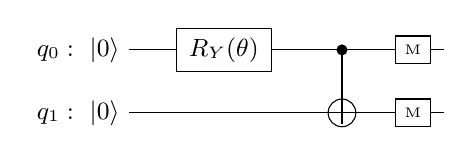
\begin{tikzpicture}[x=1cm, y=0.8cm, font=\small]
\draw (0,0) node[left]{$q_0:\ \ket0$} -- (4,0); \draw (0,-1) node[left]{$q_1:\ \ket0$} -- (4,-1);
\node[draw, fill=white, minimum width=1.2cm] at (1.2,0) {$R_Y(\theta)$};
\fill (2.7,0) circle (2pt); \draw (2.7,0) -- (2.7,-1.18); \draw (2.7,-1) circle (5pt);
\node[draw, fill=white] at (3.6,0) {\tiny M}; \node[draw, fill=white] at (3.6,-1) {\tiny M};
\end{tikzpicture}
\end{center}
Both qubits are then measured in the computational basis; $0 \le \theta \le \pi$.
\end{passagebox}
\needspace{7\baselineskip}
\begin{qitem}{39}
The expectation values $\langle Z_1\rangle$ and $\langle Z_0Z_1\rangle$ of the final state are
\par\smallskip\noindent\begin{tabularx}{\linewidth}{@{}*{4}{L}@{}}
\optlabel{A}\,$\cos\theta$ and $1$ & \optlabel{B}\,$1$ and $\cos\theta$ & \optlabel{C}\,$\cos^2(\theta/2)$ and $1$ & \optlabel{D}\,$\cos\theta$ and $\cos^2\theta$
\end{tabularx}
\end{qitem}
\qsep

\needspace{7\baselineskip}
\begin{qitem}{40}
The value of $\theta$ in $(0, \pi]$ at which the two qubits are \emph{maximally} entangled, and the purity
$\operatorname{tr}\rho_1^2$ of the reduced state of qubit 1 at that value, are
\par\smallskip\noindent\begin{tabularx}{\linewidth}{@{}*{2}{L}@{}}
\optlabel{A}\,$\theta = \pi/2$ and $\operatorname{tr}\rho_1^2 = 1$ & \optlabel{B}\,$\theta = \pi/2$ and $\operatorname{tr}\rho_1^2 = \tfrac12$ \\[3pt]
\optlabel{C}\,$\theta = \pi$ and $\operatorname{tr}\rho_1^2 = \tfrac12$ & \optlabel{D}\,$\theta = \pi/4$ and $\operatorname{tr}\rho_1^2 = \tfrac34$
\end{tabularx}
\end{qitem}
\qsep

\newpage

\begin{sectionbanner}SECTION C \enspace$\cdot$\enspace Quantum Machine Learning Fundamentals \hfill Q.41--60\end{sectionbanner}

{\small \textbf{Syllabus:} basis, angle and amplitude encoding, feature maps and quantum kernels, swap test, variational circuits, VQC, QNN and QCNN architectures, parameter-shift rule, data re-uploading, hybrid training and the QCNN of \texttt{QML.ipynb}.\\ \textbf{Formats:} Single-correct MCQ (Q.41--54); Matching lists (Q.55--56); Assertion--Reason (Q.57); Statement I / II (Q.58); Paragraph based (Q.59--60). Each question: $+3$ / $0$ / $-1$.}
\par\medskip

\needspace{7\baselineskip}
\begin{qitem}{41}
\texttt{QML.ipynb} encodes a pixel value $x \in [0, 1]$ with \texttt{ry(np.pi * x, q)} on a qubit in $\ket0$. For a
pixel of brightness $x = \frac13$ the probability of measuring $1$ on that qubit and its $\langle Z\rangle$ (before any other gate) are
\par\smallskip\noindent\begin{tabularx}{\linewidth}{@{}*{2}{L}@{}}
\optlabel{A}\,$P(1) = \frac14$, $\langle Z\rangle = \frac12$ & \optlabel{B}\,$P(1) = \frac12$, $\langle Z\rangle = 0$ \\[3pt]
\optlabel{C}\,$P(1) = \frac13$, $\langle Z\rangle = \frac13$ & \optlabel{D}\,$P(1) = \frac34$, $\langle Z\rangle = -\frac12$
\end{tabularx}
\end{qitem}
\qsep

\needspace{7\baselineskip}
\begin{qitem}{42}
The vector $\mathbf x = (1, 2, 4, 2)$ is amplitude-encoded: $\ket{\psi_{\mathbf x}} = \sum_j \frac{x_j}{\|\mathbf x\|}\ket j$ with
$\ket0 = \ket{00}, \ket1 = \ket{01}, \ket2 = \ket{10}, \ket3 = \ket{11}$ (qubit 0 written first). The number of qubits and the
probability that a measurement of qubit 0 gives 1 are
\par\smallskip\noindent\begin{tabularx}{\linewidth}{@{}*{4}{L}@{}}
\optlabel{A}\,$2$ qubits; $0.32$ & \optlabel{B}\,$2$ qubits; $0.60$ & \optlabel{C}\,$4$ qubits; $0.80$ & \optlabel{D}\,$2$ qubits; $0.80$
\end{tabularx}
\end{qitem}
\qsep

\needspace{7\baselineskip}
\begin{qitem}{43}
A data point has $d = 256$ real features, each stored with 8-bit precision. The numbers of qubits needed by
\emph{basis} encoding (every bit on its own qubit), \emph{angle} encoding (one feature per qubit) and \emph{amplitude} encoding are
\par\smallskip\noindent\begin{tabularx}{\linewidth}{@{}*{4}{L}@{}}
\optlabel{A}\,$256$, $256$, $8$ & \optlabel{B}\,$8$, $256$, $2048$ & \optlabel{C}\,$2048$, $256$, $8$ & \optlabel{D}\,$2048$, $8$, $256$
\end{tabularx}
\end{qitem}
\qsep

\needspace{7\baselineskip}
\begin{qitem}{44}
With the notebook's angle encoding $\ket{\psi(\mathbf x)} = \bigotimes_i R_Y(\pi x_i)\ket0$, the fidelity (quantum) kernel
$k(\mathbf x, \mathbf x') = |\braket{\psi(\mathbf x)|\psi(\mathbf x')}|^2$ for $\mathbf x = (1, 0.5)$ and $\mathbf x' = (0.5, 0)$ is
\par\smallskip\noindent\begin{tabularx}{\linewidth}{@{}*{4}{L}@{}}
\optlabel{A}\,$\frac1{16}$ & \optlabel{B}\,$\frac14$ & \optlabel{C}\,$\frac12$ & \optlabel{D}\,$0$
\end{tabularx}
\end{qitem}
\qsep

\needspace{7\baselineskip}
\begin{qitem}{45}
A quantum-kernel SVM is trained on $M = 20$ points. Every kernel entry $k_{ij} = |\braket{\psi_i|\psi_j}|^2$, with $\ket{\psi_i} = \ket{\psi(\mathbf x_i)}$,
is estimated by its own circuit. Using $k(\mathbf x, \mathbf x) = 1$ and the symmetry $k_{ij} = k_{ji}$, the number of distinct
circuits needed for the training Gram matrix is
\par\smallskip\noindent\begin{tabularx}{\linewidth}{@{}*{4}{L}@{}}
\optlabel{A}\,$190$ & \optlabel{B}\,$400$ & \optlabel{C}\,$380$ & \optlabel{D}\,$20$
\end{tabularx}
\end{qitem}
\qsep

\needspace{7\baselineskip}
\begin{qitem}{46}
In a swap test between the states $\ket\psi$ and $\ket\phi$ the ancilla is measured in state $0$ with probability $0.8$.
The fidelity kernel $|\braket{\psi|\phi}|^2$ is
\par\smallskip\noindent\begin{tabularx}{\linewidth}{@{}*{4}{L}@{}}
\optlabel{A}\,$0.3$ & \optlabel{B}\,$0.8$ & \optlabel{C}\,$0.89$ & \optlabel{D}\,$0.6$
\end{tabularx}
\end{qitem}
\qsep

\needspace{7\baselineskip}
\begin{qitem}{47}
A parameter $\theta$ enters a circuit only through one gate $R_Y(\theta)$. The measured expectation values are
$f(\theta + \frac\pi2) = 0.30$ and $f(\theta - \frac\pi2) = -0.50$. The exact derivative $f'(\theta)$ is
\par\smallskip\noindent\begin{tabularx}{\linewidth}{@{}*{4}{L}@{}}
\optlabel{A}\,$-0.40$ & \optlabel{B}\,$0.25$ & \optlabel{C}\,$0.40$ & \optlabel{D}\,$0.80$
\end{tabularx}
\end{qitem}
\qsep

\needspace{7\baselineskip}
\begin{qitem}{48}
In the default 8-qubit QCNN of \texttt{QML.ipynb}, the parameter $\theta_{1,1}$ = \texttt{theta[0]} is used by how many
$R_Y$ gates, and how many circuit evaluations does an exact parameter-shift derivative with respect to it need for one image
(shifting each occurrence separately)?
\par\smallskip\noindent\begin{tabularx}{\linewidth}{@{}*{2}{L}@{}}
\optlabel{A}\,$11$ gates; $22$ circuits & \optlabel{B}\,$4$ gates; $8$ circuits \\[3pt]
\optlabel{C}\,$7$ gates; $14$ circuits & \optlabel{D}\,$1$ gate; $2$ circuits
\end{tabularx}
\end{qitem}
\qsep

\needspace{7\baselineskip}
\begin{qitem}{49}
Using the notebook's layout rule (pool pairs of active qubits, keep the sinks; an odd last qubit moves on unchanged;
4 parameters per layer), a QCNN on $N = 20$ qubits (e.g.\ $4\times5$ pixels) has
\par\smallskip\noindent\begin{tabularx}{\linewidth}{@{}*{2}{L}@{}}
\optlabel{A}\,$4$ layers and $16$ parameters & \optlabel{B}\,$19$ layers and $76$ parameters \\[3pt]
\optlabel{C}\,$5$ layers and $40$ parameters & \optlabel{D}\,$5$ layers and $20$ parameters
\end{tabularx}
\end{qitem}
\qsep

\needspace{7\baselineskip}
\begin{qitem}{50}
The pooling block of \texttt{QML.ipynb} on source qubit $a$ and sink qubit $b$ is
\texttt{rz.ctrl(t3, q[a], q[b]); x(q[a]); rx.ctrl(t4, q[a], q[b]); x(q[a])}. As an operator it equals
\par\smallskip\noindent\begin{tabularx}{\linewidth}{@{}*{2}{L}@{}}
\optlabel{A}\,$R_Z(t_3)_b\,R_X(t_4)_b$ (independent of qubit $a$) & \optlabel{B}\,$\ket1\!\bra1_b\otimes R_Z(t_3)_a + \ket0\!\bra0_b\otimes R_X(t_4)_a$ \\[3pt]
\optlabel{C}\,$\ket0\!\bra0_a\otimes R_Z(t_3)_b + \ket1\!\bra1_a\otimes R_X(t_4)_b$ & \optlabel{D}\,$\ket1\!\bra1_a\otimes R_Z(t_3)_b + \ket0\!\bra0_a\otimes R_X(t_4)_b$
\end{tabularx}
\end{qitem}
\qsep

\needspace{7\baselineskip}
\begin{qitem}{51}
For $N = 16$ qubits the notebook's layout has $26$ convolution blocks and $15$ pooling blocks. Counting the $N$
encoding rotations and every gate of the blocks as \texttt{cudaq.estimate\_resources} does, the circuit has
\par\smallskip\noindent\begin{tabularx}{\linewidth}{@{}*{4}{L}@{}}
\optlabel{A}\,$138$ gates & \optlabel{B}\,$154$ gates & \optlabel{C}\,$124$ gates & \optlabel{D}\,$170$ gates
\end{tabularx}
\end{qitem}
\qsep

\needspace{7\baselineskip}
\begin{qitem}{52}
A classifier with outputs in $[-1, 1]$ and prediction $\operatorname{sign} f$ gives $f = 0.6,\ -0.2,\ 0.9,\ 0.1$ on four
images with labels $y = +1,\ -1,\ +1,\ -1$. Its mean squared error (as in \texttt{QML.ipynb}) and accuracy are
\par\smallskip\noindent\begin{tabularx}{\linewidth}{@{}*{4}{L}@{}}
\optlabel{A}\,$0.505$ and $75\,\%$ & \optlabel{B}\,$2.02$ and $75\,\%$ & \optlabel{C}\,$0.60$ and $75\,\%$ & \optlabel{D}\,$0.505$ and $50\,\%$
\end{tabularx}
\end{qitem}
\qsep

\needspace{7\baselineskip}
\begin{qitem}{53}
With its defaults (20 training images, \texttt{MAX\_ITERATIONS = 100} loss evaluations, 20 test images) and the
recorded time of $1.7$ ms per circuit on \texttt{qpp-cpu}, the number of circuits \texttt{QML.ipynb} runs for training plus testing
and the resulting estimate of the run time are
\par\smallskip\noindent\begin{tabularx}{\linewidth}{@{}*{2}{L}@{}}
\optlabel{A}\,$2020$ circuits, about $3.4$ s & \optlabel{B}\,$100$ circuits, about $0.17$ s \\[3pt]
\optlabel{C}\,$2020$ circuits, about $34$ s & \optlabel{D}\,$2000$ circuits, about $0.17$ s
\end{tabularx}
\end{qitem}
\qsep

\needspace{7\baselineskip}
\begin{qitem}{54}
A single-qubit model alternates trainable unitaries with the data-encoding gate $R_Y(x)$, which appears $L = 3$ times
(``data re-uploading''). Its output $f(x) = \langle Z\rangle$ is a trigonometric series in $x$. The highest frequency it can contain is
\par\smallskip\noindent\begin{tabularx}{\linewidth}{@{}*{4}{L}@{}}
\optlabel{A}\,$8$ & \optlabel{B}\,$3$ & \optlabel{C}\,$1$ & \optlabel{D}\,$6$
\end{tabularx}
\end{qitem}
\qsep

\needspace{7\baselineskip}
\begin{qitem}{55}
Match each data encoding (List-I) with its description (List-II); $d$ = number of features.
\par\smallskip\noindent{\renewcommand{\arraystretch}{1.35}%
\begin{tabularx}{\linewidth}{@{}c>{\raggedright\arraybackslash}p{0.33\linewidth}@{\hspace{1.2em}}cL@{}}
\toprule
\multicolumn{2}{@{}l}{\textbf{List-I}} & \multicolumn{2}{l@{}}{\textbf{List-II}} \\ \midrule
\textbf{(P)} & basis encoding of a $d$-bit string & \textbf{(1)} & $\log_2 d$ qubits; preparing a general state needs $O(d)$ gates \\
\textbf{(Q)} & angle encoding $\bigotimes_i R_Y(x_i)\ket0$ & \textbf{(2)} & $d$ qubits; an $X$ gate on every qubit whose bit is 1; basis states only \\
\textbf{(R)} & amplitude encoding of $d = 2^n$ real numbers & \textbf{(3)} & $d$ qubits; Hadamards, then phases $e^{-i\phi_i(\mathbf x)Z_i}$ and $e^{-i\phi_{ij}(\mathbf x)Z_iZ_j}$; entangling; conjectured hard to simulate classically \\
\textbf{(S)} & ZZ (IQP-type) feature map & \textbf{(4)} & $d$ qubits; depth 1; product state, so its kernel factorises \\
\bottomrule
\end{tabularx}}
\par\smallskip\noindent\begin{tabularx}{\linewidth}{@{}*{2}{L}@{}}
\optlabel{A}\,P$\to$1, Q$\to$4, R$\to$2, S$\to$3 & \optlabel{B}\,P$\to$4, Q$\to$2, R$\to$1, S$\to$3 \\[3pt]
\optlabel{C}\,P$\to$2, Q$\to$4, R$\to$1, S$\to$3 & \optlabel{D}\,P$\to$2, Q$\to$4, R$\to$3, S$\to$1
\end{tabularx}
\end{qitem}
\qsep

\needspace{7\baselineskip}
\begin{qitem}{56}
Match each QML model (List-I) with what is trained (List-II).
\par\smallskip\noindent{\renewcommand{\arraystretch}{1.35}%
\begin{tabularx}{\linewidth}{@{}c>{\raggedright\arraybackslash}p{0.33\linewidth}@{\hspace{1.2em}}cL@{}}
\toprule
\multicolumn{2}{@{}l}{\textbf{List-I}} & \multicolumn{2}{l@{}}{\textbf{List-II}} \\ \midrule
\textbf{(P)} & quantum-kernel SVM & \textbf{(1)} & a parameterised generator circuit, trained adversarially against a discriminator \\
\textbf{(Q)} & variational quantum classifier (VQC) & \textbf{(2)} & no circuit parameters: the feature map is fixed; the classical dual coefficients $\alpha_m$ are trained \\
\textbf{(R)} & QCNN & \textbf{(3)} & a feature map followed by a trainable ansatz $U(\boldsymbol\theta)$; $\boldsymbol\theta$ is updated by a classical optimizer \\
\textbf{(S)} & quantum GAN & \textbf{(4)} & convolution and pooling layers with shared parameters; $O(\log N)$ parameters; one output qubit \\
\bottomrule
\end{tabularx}}
\par\smallskip\noindent\begin{tabularx}{\linewidth}{@{}*{2}{L}@{}}
\optlabel{A}\,P$\to$3, Q$\to$2, R$\to$4, S$\to$1 & \optlabel{B}\,P$\to$2, Q$\to$3, R$\to$1, S$\to$4 \\[3pt]
\optlabel{C}\,P$\to$2, Q$\to$3, R$\to$4, S$\to$1 & \optlabel{D}\,P$\to$2, Q$\to$4, R$\to$3, S$\to$1
\end{tabularx}
\end{qitem}
\qsep

\needspace{7\baselineskip}
\begin{qitem}{57}
\textbf{Assertion (A):} \texttt{QML.ipynb} trains its QCNN without evaluating any gradient circuits.\\[1mm]
\textbf{Reason (R):} Several QCNN parameters enter controlled rotations (\texttt{rz.ctrl}, \texttt{rx.ctrl}), for which the two-term
parameter-shift rule with shifts $\pm\frac\pi2$ is not exact.
\begin{itemize}[leftmargin=2.6em, labelsep=0.4em, itemsep=2pt, topsep=3pt]
\item[\optlabel{A}] Both Assertion (A) and Reason (R) are true, and R is the correct explanation of A
\item[\optlabel{B}] Both A and R are true, but R is \emph{not} the correct explanation of A
\item[\optlabel{C}] A is true, but R is false
\item[\optlabel{D}] A is false, but R is true
\end{itemize}
\end{qitem}
\qsep

\needspace{7\baselineskip}
\begin{qitem}{58}
\textbf{Statement I:} For any feature map, the exact Gram matrix $K_{ij} = |\braket{\psi(\mathbf x_i)|\psi(\mathbf x_j)}|^2$ is
symmetric and positive semi-definite.\\[1mm]
\textbf{Statement II:} When the entries $K_{ij}$ are \emph{estimated} with a finite number of shots, the estimated matrix can have small
negative eigenvalues.
\begin{itemize}[leftmargin=2.6em, labelsep=0.4em, itemsep=2pt, topsep=3pt]
\item[\optlabel{A}] Both Statement I and Statement II are true
\item[\optlabel{B}] Both Statement I and Statement II are false
\item[\optlabel{C}] Statement I is true, but Statement II is false
\item[\optlabel{D}] Statement I is false, but Statement II is true
\end{itemize}
\end{qitem}
\qsep

\needspace{20\baselineskip}
\begin{passagebox}{Paragraph for Questions 59 and 60}
A two-qubit variational quantum classifier (VQC) encodes the features $(x_0, x_1)$ with $R_Y(x_0)$ on qubit 0 and
$R_Y(x_1)$ on qubit 1, applies a CNOT (control 0, target 1) and then one trainable gate $R_Y(\theta)$ on qubit 1. Its output
is $f(\mathbf x; \theta) = \langle Z_1\rangle$, the prediction is $\operatorname{sign} f$, and the loss of one example is $L = (f - y)^2$.
\begin{center}
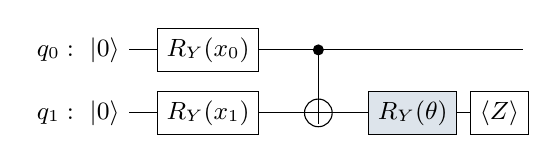
\begin{tikzpicture}[x=1cm, y=0.8cm, font=\small]
\draw (0,0) node[left]{$q_0:\ \ket0$} -- (5,0); \draw (0,-1) node[left]{$q_1:\ \ket0$} -- (5,-1);
\node[draw, fill=white] at (1,0) {$R_Y(x_0)$}; \node[draw, fill=white] at (1,-1) {$R_Y(x_1)$};
\fill (2.4,0) circle (2pt); \draw (2.4,0) -- (2.4,-1.18); \draw (2.4,-1) circle (5pt);
\node[draw, fill=brand!15] at (3.6,-1) {$R_Y(\theta)$}; \node[draw, fill=white] at (4.7,-1) {$\langle Z\rangle$};
\end{tikzpicture}
\end{center}
\end{passagebox}
\needspace{7\baselineskip}
\begin{qitem}{59}
The model output $f(\mathbf x; \theta) = \langle Z_1\rangle$ equals
\par\smallskip\noindent\begin{tabularx}{\linewidth}{@{}*{2}{L}@{}}
\optlabel{A}\,$\cos\theta\cos x_1 - \sin\theta\sin x_0\sin x_1$ & \optlabel{B}\,$\cos\theta\cos x_0\cos x_1 - \sin\theta\sin x_1$ \\[3pt]
\optlabel{C}\,$\cos\theta\cos x_0\cos x_1 + \sin\theta\sin x_1$ & \optlabel{D}\,$\cos(\theta + x_1)\cos x_0$
\end{tabularx}
\end{qitem}
\qsep

\needspace{7\baselineskip}
\begin{qitem}{60}
For $\mathbf x = (0, \frac\pi3)$, $\theta = \frac\pi6$ and label $y = +1$, the shifted outputs $f(\theta + \frac\pi2)$, $f(\theta - \frac\pi2)$ and
the loss gradient $\partial L/\partial\theta$ are
\par\smallskip\noindent\begin{tabularx}{\linewidth}{@{}*{4}{L}@{}}
\optlabel{A}\,$+1,\ -1,\ +2$ & \optlabel{B}\,$-1,\ +1,\ -2$ & \optlabel{C}\,$-1,\ +1,\ -1$ & \optlabel{D}\,$-1,\ +1,\ +2$
\end{tabularx}
\end{qitem}
\qsep

\newpage

\begin{sectionbanner}SECTION D \enspace$\cdot$\enspace Advanced QML and Implementation \hfill Q.61--80\end{sectionbanner}

{\small \textbf{Syllabus:} barren plateaus, generalised shift rules and gradient cost, noise, kernel concentration, quantum SVM, qPCA, QGAN, quantum RL and clustering, CUDA-Q targets and GPU memory, model evaluation, benchmarking against classical baselines, limitations and interpretation of recorded results.\\ \textbf{Formats:} Single-correct MCQ (Q.61--74); Matching lists (Q.75--76); Assertion--Reason (Q.77); Statement I / II (Q.78); Paragraph based (Q.79--80). Each question: $+3$ / $0$ / $-1$.}
\par\medskip

\needspace{7\baselineskip}
\begin{qitem}{61}
For a deep random circuit with a global cost function the gradient components satisfy $\mathbb E[\partial_kC] = 0$ and
$\operatorname{Var}[\partial_kC] \approx 2^{-n}$. Each cost value is estimated with $S$ shots (statistical error $\approx 1/\sqrt S$). To resolve a
typical gradient component at $n = 20$ qubits one needs roughly
\par\smallskip\noindent\begin{tabularx}{\linewidth}{@{}*{4}{L}@{}}
\optlabel{A}\,$S \sim 20$ shots & \optlabel{B}\,$S \sim 10^{6}$ shots & \optlabel{C}\,$S \sim 10^{12}$ shots & \optlabel{D}\,$S \sim 400$ shots
\end{tabularx}
\end{qitem}
\qsep

\needspace{7\baselineskip}
\begin{qitem}{62}
Which statement about barren plateaus is correct?
\begin{itemize}[leftmargin=2.6em, labelsep=0.4em, itemsep=2pt, topsep=3pt]
\item[\optlabel{A}] For random circuits deep enough to form approximate 2-designs, gradient variances vanish exponentially in $n$; for shallow circuits, local cost functions have only polynomially vanishing gradients while global cost functions can still vanish exponentially.
\item[\optlabel{B}] Barren plateaus are caused only by hardware noise, so they never appear in noiseless simulation.
\item[\optlabel{C}] Switching to a gradient-free optimizer such as COBYLA removes a barren plateau, because no gradients are computed.
\item[\optlabel{D}] A barren plateau can be removed by multiplying the learning rate by $2^n$.
\end{itemize}
\end{qitem}
\qsep

\needspace{7\baselineskip}
\begin{qitem}{63}
In a Hadamard test with a controlled-$R_Z(\theta)$ the measured output is $f(\theta) = \cos(\theta/2)$ (a pure frequency
$\frac12$). At $\theta = \pi$, the two-term shift formula $\frac12[f(\theta + \frac\pi2) - f(\theta - \frac\pi2)]$ and the exact derivative $f'(\pi)$ are
\par\smallskip\noindent\begin{tabularx}{\linewidth}{@{}*{2}{L}@{}}
\optlabel{A}\,$-0.707$ and $-0.5$ & \optlabel{B}\,$-0.5$ and $-0.5$ \\[3pt]
\optlabel{C}\,$-1$ and $-0.5$ & \optlabel{D}\,$-0.707$ and $-0.707$
\end{tabularx}
\end{qitem}
\qsep

\needspace{7\baselineskip}
\begin{qitem}{64}
In a simple global-depolarising model every gate multiplies the output expectation value by $(1 - p)$. For the default
QCNN (69 gates) and $p = 0.01$, the expectation values are multiplied by about ..., and the test \emph{accuracy} (prediction
$\operatorname{sign}\langle Z\rangle$) is expected to
\begin{itemize}[leftmargin=2.6em, labelsep=0.4em, itemsep=2pt, topsep=3pt]
\item[\optlabel{A}] $0.31$; drop to $50\,\%$
\item[\optlabel{B}] $0.50$; stay the same, while $|\langle Z\rangle|$ shrinks and the MSE grows
\item[\optlabel{C}] $0.50$; drop to about $50\,\%$, because half of the predictions flip sign
\item[\optlabel{D}] $0.99$; stay the same, and noise is negligible
\end{itemize}
\end{qitem}
\qsep

\needspace{7\baselineskip}
\begin{qitem}{65}
An 80 GB GPU simulates state vectors in double precision (16 bytes per amplitude). The largest number of qubits that
fits on one GPU, and on four such GPUs pooled for one distributed state vector, are
\par\smallskip\noindent\begin{tabularx}{\linewidth}{@{}*{4}{L}@{}}
\optlabel{A}\,$36$ and $38$ & \optlabel{B}\,$32$ and $128$ & \optlabel{C}\,$33$ and $35$ & \optlabel{D}\,$32$ and $34$
\end{tabularx}
\end{qitem}
\qsep

\needspace{7\baselineskip}
\begin{qitem}{66}
Suppose the 8-qubit QCNN (11 convolution blocks, 7 pooling blocks) were trained by gradient descent with \emph{exact}
parameter-shift gradients: every $R_Y$ occurrence shifted separately (2 circuits), every controlled rotation (\texttt{crz}, \texttt{crx})
with the four-term rule (4 circuits). The number of circuits for \emph{one} full gradient of the loss over the 20 training images is
\par\smallskip\noindent\begin{tabularx}{\linewidth}{@{}*{4}{L}@{}}
\optlabel{A}\,$480$ & \optlabel{B}\,$1440$ & \optlabel{C}\,$40$ & \optlabel{D}\,$2000$
\end{tabularx}
\end{qitem}
\qsep

\needspace{7\baselineskip}
\begin{qitem}{67}
\texttt{cudaq.sample} on a two-qubit kernel returns the counts \texttt{\{'00': 400, '01': 100, '10': 300, '11': 200\}}
(the first character is qubit 0). The estimates of $\big(\langle Z_0\rangle, \langle Z_1\rangle, \langle Z_0Z_1\rangle\big)$ are
\par\smallskip\noindent\begin{tabularx}{\linewidth}{@{}*{4}{L}@{}}
\optlabel{A}\,$(0,\ 0.4,\ 0.2)$ & \optlabel{B}\,$(0,\ 0.4,\ 0)$ & \optlabel{C}\,$(0,\ 0.4,\ 0.6)$ & \optlabel{D}\,$(0.4,\ 0,\ 0.2)$
\end{tabularx}
\end{qitem}
\qsep

\needspace{7\baselineskip}
\begin{qitem}{68}
The recorded run of \texttt{QML.ipynb} ends with training accuracy $90\,\%$ but training MSE $0.67$ (the mean
$|\langle Z_7\rangle|$ of the trained model on the training images is about $0.20$). The best explanation is
\begin{itemize}[leftmargin=2.6em, labelsep=0.4em, itemsep=2pt, topsep=3pt]
\item[\optlabel{A}] the outputs have the correct sign but small magnitude, so each correct image still contributes about $(1 - 0.2)^2 = 0.64$ to the loss
\item[\optlabel{B}] a bug: for $\pm1$ labels the MSE must equal $1 - \text{accuracy} = 0.10$
\item[\optlabel{C}] COBYLA diverged in the last iterations, so the loss and the accuracy belong to different parameter vectors
\item[\optlabel{D}] the MSE is computed on the test images, the accuracy on the training images
\end{itemize}
\end{qitem}
\qsep

\needspace{7\baselineskip}
\begin{qitem}{69}
The README of the repository reports a 15-qubit test of \texttt{QML.ipynb} ($3\times5$ images, 16 training images, 60 COBYLA
evaluations) at about $0.35$ s per circuit on the 4-core test CPU. The training time is about
\par\smallskip\noindent\begin{tabularx}{\linewidth}{@{}*{4}{L}@{}}
\optlabel{A}\,$21$ seconds & \optlabel{B}\,$5.6$ minutes & \optlabel{C}\,$0.35$ seconds & \optlabel{D}\,$56$ minutes
\end{tabularx}
\end{qitem}
\qsep

\needspace{7\baselineskip}
\begin{qitem}{70}
For the product kernel $k(\mathbf x, \mathbf x') = \prod_{i=1}^{n}\cos^2\frac{\pi(x_i - x'_i)}{2}$ with all $x_i, x'_i$ independent
and uniform on $[0, 1]$, the average off-diagonal kernel value $\mathbb E[k]$ equals
\par\smallskip\noindent\begin{tabularx}{\linewidth}{@{}*{2}{L}@{}}
\optlabel{A}\,$(2/\pi)^n$ & \optlabel{B}\,$2^{-n}$ \\[3pt]
\optlabel{C}\,$\big(\tfrac12 + \tfrac{2}{\pi^2}\big)^n \approx 0.70^n$ & \optlabel{D}\,$1/n$
\end{tabularx}
\end{qitem}
\qsep

\needspace{7\baselineskip}
\begin{qitem}{71}
Which statement about quantum principal component analysis (qPCA, Lloyd, Mohseni \& Rebentrost 2014) is correct?
\begin{itemize}[leftmargin=2.6em, labelsep=0.4em, itemsep=2pt, topsep=3pt]
\item[\optlabel{A}] It uses many copies of a density matrix $\rho$ to apply $e^{-i\rho t}$ (density-matrix exponentiation) and phase estimation to reveal its large eigenvalues; the output is a quantum state, and any speed-up assumes efficient state preparation and low rank --- dequantized classical algorithms match it under comparable assumptions.
\item[\optlabel{B}] It is the pooling layer of the QCNN in \texttt{QML.ipynb}.
\item[\optlabel{C}] It diagonalises the covariance matrix of $N$ classical data points in $O(\log N)$ total time, including loading the data and reading out all eigenvectors.
\item[\optlabel{D}] It needs only a single copy of $\rho$, because one measurement reveals all eigenvalues.
\end{itemize}
\end{qitem}
\qsep

\needspace{7\baselineskip}
\begin{qitem}{72}
A (quantum or classical) GAN optimises $V(D, G) = \mathbb E_{x\sim p_{\text{data}}}[\ln D(x)] + \mathbb E_{x\sim p_G}[\ln(1 - D(x))]$.
At the ideal equilibrium $p_G = p_{\text{data}}$ with the optimal discriminator, the value of $V$ is
\par\smallskip\noindent\begin{tabularx}{\linewidth}{@{}*{4}{L}@{}}
\optlabel{A}\,$0$ & \optlabel{B}\,$-\tfrac12$ & \optlabel{C}\,$-\ln 4 \approx -1.386$ & \optlabel{D}\,$\ln 2$
\end{tabularx}
\end{qitem}
\qsep

\needspace{7\baselineskip}
\begin{qitem}{73}
In (quantum) reinforcement learning with Q-learning, $Q(s, a) \leftarrow Q(s, a) + \alpha\big[r + \gamma\max_{a'}Q(s', a') - Q(s, a)\big]$.
With $Q(s, a) = 2$, $\alpha = 0.5$, reward $r = 1$, discount $\gamma = 0.9$ and $\max_{a'}Q(s', a') = 4$, the updated value is
\par\smallskip\noindent\begin{tabularx}{\linewidth}{@{}*{4}{L}@{}}
\optlabel{A}\,$3.5$ & \optlabel{B}\,$2.6$ & \optlabel{C}\,$3.3$ & \optlabel{D}\,$4.6$
\end{tabularx}
\end{qitem}
\qsep

\needspace{7\baselineskip}
\begin{qitem}{74}
A quantum clustering algorithm estimates distances between normalised real data vectors $\mathbf a, \mathbf b$ with a swap test.
The ancilla gives $0$ with probability $0.9$, and $\mathbf a\cdot\mathbf b > 0$ is known. The Euclidean distance $\|\mathbf a - \mathbf b\|$ is about
\par\smallskip\noindent\begin{tabularx}{\linewidth}{@{}*{4}{L}@{}}
\optlabel{A}\,$0.21$ & \optlabel{B}\,$0.46$ & \optlabel{C}\,$0.63$ & \optlabel{D}\,$0.89$
\end{tabularx}
\end{qitem}
\qsep

\needspace{7\baselineskip}
\begin{qitem}{75}
Match each CUDA-Q target (List-I) with its use (List-II).
\par\smallskip\noindent{\renewcommand{\arraystretch}{1.35}%
\begin{tabularx}{\linewidth}{@{}c>{\raggedright\arraybackslash}p{0.33\linewidth}@{\hspace{1.2em}}cL@{}}
\toprule
\multicolumn{2}{@{}l}{\textbf{List-I}} & \multicolumn{2}{l@{}}{\textbf{List-II}} \\ \midrule
\textbf{(P)} & \texttt{qpp-cpu} & \textbf{(1)} & one state vector distributed over several GPUs (one MPI rank per GPU) to simulate more qubits \\
\textbf{(Q)} & \texttt{nvidia} with option \texttt{mgpu} & \textbf{(2)} & several independent virtual QPUs (one per GPU) that run \emph{different} circuits in parallel, e.g.\ many images or shift terms \\
\textbf{(R)} & \texttt{nvidia} with option \texttt{mqpu} & \textbf{(3)} & CPU state-vector simulator; produced the recorded outputs of \texttt{QML.ipynb} \\
\textbf{(S)} & \texttt{density-matrix-cpu} & \textbf{(4)} & noisy simulation with a noise model; memory $16\cdot4^N$ bytes \\
\bottomrule
\end{tabularx}}
\par\smallskip\noindent\begin{tabularx}{\linewidth}{@{}*{2}{L}@{}}
\optlabel{A}\,P$\to$3, Q$\to$1, R$\to$4, S$\to$2 & \optlabel{B}\,P$\to$4, Q$\to$1, R$\to$2, S$\to$3 \\[3pt]
\optlabel{C}\,P$\to$3, Q$\to$1, R$\to$2, S$\to$4 & \optlabel{D}\,P$\to$3, Q$\to$2, R$\to$1, S$\to$4
\end{tabularx}
\end{qitem}
\qsep

\needspace{7\baselineskip}
\begin{qitem}{76}
Match each limitation of QML (List-I) with its description (List-II).
\par\smallskip\noindent{\renewcommand{\arraystretch}{1.35}%
\begin{tabularx}{\linewidth}{@{}c>{\raggedright\arraybackslash}p{0.33\linewidth}@{\hspace{1.2em}}cL@{}}
\toprule
\multicolumn{2}{@{}l}{\textbf{List-I}} & \multicolumn{2}{l@{}}{\textbf{List-II}} \\ \midrule
\textbf{(P)} & barren plateau & \textbf{(1)} & classical sampling algorithms reproduce claimed exponential speed-ups (e.g.\ recommendation systems, PCA) under the same input assumptions \\
\textbf{(Q)} & dequantization & \textbf{(2)} & the variance of cost gradients decays exponentially with the number of qubits \\
\textbf{(R)} & data-loading bottleneck & \textbf{(3)} & off-diagonal kernel values approach a constant exponentially fast, so exponentially many shots are needed to distinguish them \\
\textbf{(S)} & exponential kernel concentration & \textbf{(4)} & preparing a general amplitude-encoded state of $2^n$ numbers needs $O(2^n)$ gates, which can cancel a speed-up \\
\bottomrule
\end{tabularx}}
\par\smallskip\noindent\begin{tabularx}{\linewidth}{@{}*{2}{L}@{}}
\optlabel{A}\,P$\to$2, Q$\to$4, R$\to$1, S$\to$3 & \optlabel{B}\,P$\to$1, Q$\to$2, R$\to$4, S$\to$3 \\[3pt]
\optlabel{C}\,P$\to$3, Q$\to$1, R$\to$4, S$\to$2 & \optlabel{D}\,P$\to$2, Q$\to$1, R$\to$4, S$\to$3
\end{tabularx}
\end{qitem}
\qsep

\needspace{7\baselineskip}
\begin{qitem}{77}
\textbf{Assertion (A):} Because the QCNN of \texttt{QML.ipynb} reaches $85\,\%$ test accuracy, it demonstrates a quantum advantage
over classical image classifiers.\\[1mm]
\textbf{Reason (R):} Before any advantage can be claimed, the quantum model must be compared with classical baselines trained and
evaluated on the same data, at comparable cost.
\begin{itemize}[leftmargin=2.6em, labelsep=0.4em, itemsep=2pt, topsep=3pt]
\item[\optlabel{A}] Both Assertion (A) and Reason (R) are true, and R is the correct explanation of A
\item[\optlabel{B}] Both A and R are true, but R is \emph{not} the correct explanation of A
\item[\optlabel{C}] A is true, but R is false
\item[\optlabel{D}] A is false, but R is true
\end{itemize}
\end{qitem}
\qsep

\needspace{7\baselineskip}
\begin{qitem}{78}
\textbf{Statement I:} The outputs stored in \texttt{QML.ipynb} were produced on an NVIDIA GPU.\\[1mm]
\textbf{Statement II:} With \texttt{TARGET = "auto"} on a machine with two GPUs, \texttt{QML.ipynb} distributes the QCNN state vector over both GPUs.
\begin{itemize}[leftmargin=2.6em, labelsep=0.4em, itemsep=2pt, topsep=3pt]
\item[\optlabel{A}] Both Statement I and Statement II are true
\item[\optlabel{B}] Both Statement I and Statement II are false
\item[\optlabel{C}] Statement I is true, but Statement II is false
\item[\optlabel{D}] Statement I is false, but Statement II is true
\end{itemize}
\end{qitem}
\qsep

\needspace{20\baselineskip}
\begin{passagebox}{Paragraph for Questions 79 and 80}
For the lecture, \texttt{QML.ipynb} was re-executed with its default settings (CUDA-Q 0.16.0, \texttt{qpp-cpu}, no GPU).
It reproduced the recorded outputs exactly: loss $1.1214 \to 0.6704$, training accuracy $90\,\%$, test accuracy $85\,\%$.
With ``horizontal'' as the positive class, the 20 test images give the confusion matrix
\begin{center}\small
\begin{tabular}{lcc}\toprule & predicted horizontal & predicted vertical\\ \midrule
true horizontal (10 images) & 9 & 1\\ true vertical (10 images) & 2 & 8\\ \bottomrule\end{tabular}
\end{center}
Further measurements on the \emph{same} 20 training images (illustrative experiments, not part of the notebook):
logistic regression on the 8 raw pixels reaches $45\,\%$ test accuracy; a hand-written rule (``is some horizontal pixel pair
brighter than every vertical pixel pair?'') reaches $100\,\%$; an SVM with the fidelity kernel of the notebook's angle encoding
reaches $100\,\%$. On $2000$ fresh images from the same generator the accuracies are: trained QCNN $80.2\,\%$, kernel SVM
$95.2\,\%$, hand-written rule $100\,\%$, logistic regression $46.5\,\%$.
\end{passagebox}
\needspace{7\baselineskip}
\begin{qitem}{79}
For the positive class ``horizontal'', the precision, recall and F1-score of the trained QCNN on the 20 test images are
\par\smallskip\noindent\begin{tabularx}{\linewidth}{@{}*{2}{L}@{}}
\optlabel{A}\,$0.900$, $0.818$, $0.857$ & \optlabel{B}\,$0.850$, $0.850$, $0.850$ \\[3pt]
\optlabel{C}\,$0.818$, $0.900$, $0.857$ & \optlabel{D}\,$0.818$, $0.900$, $0.859$
\end{tabularx}
\end{qitem}
\qsep

\needspace{7\baselineskip}
\begin{qitem}{80}
Which conclusion is supported by these measurements?
\begin{itemize}[leftmargin=2.6em, labelsep=0.4em, itemsep=2pt, topsep=3pt]
\item[\optlabel{A}] The drop from $85\,\%$ to $80.2\,\%$ proves that the 2000 fresh images come from a different distribution than the training images.
\item[\optlabel{B}] The kernel SVM result requires a quantum computer, because its kernel is defined as an overlap of quantum states.
\item[\optlabel{C}] The QCNN demonstrates a quantum advantage, because it beats logistic regression by about 35 points.
\item[\optlabel{D}] On fresh data the QCNN ($80.2\,\%$) is below the classically computable kernel SVM ($95.2\,\%$) and the simple rule ($100\,\%$); its $85\,\%$ on 20 images lies within about one standard error ($\approx8$ points) of $80\,\%$; logistic regression fails because the classes are not linearly separable in pixel space.
\end{itemize}
\end{qitem}
\qsep

\newpage

\begin{center}{\Large\bfseries\color{brand} RESPONSE SHEET}\\[2pt]
{\small Darken exactly ONE bubble per question. Leave all four bubbles empty to skip a question (0 marks).}\end{center}
\textbf{Name:} \hrulefill\quad \textbf{Roll No.:} \rule{35mm}{0.4pt}\par\medskip
\noindent\begin{minipage}[t]{0.235\linewidth}\centering
\textbf{Section A}\\[2pt]
\begin{tabular}{@{}r@{\hspace{5pt}}l@{}}
\textbf{1} & \bub{A}\,\bub{B}\,\bub{C}\,\bub{D} \\[1.6pt]
\textbf{2} & \bub{A}\,\bub{B}\,\bub{C}\,\bub{D} \\[1.6pt]
\textbf{3} & \bub{A}\,\bub{B}\,\bub{C}\,\bub{D} \\[1.6pt]
\textbf{4} & \bub{A}\,\bub{B}\,\bub{C}\,\bub{D} \\[1.6pt]
\textbf{5} & \bub{A}\,\bub{B}\,\bub{C}\,\bub{D} \\[1.6pt]
\textbf{6} & \bub{A}\,\bub{B}\,\bub{C}\,\bub{D} \\[1.6pt]
\textbf{7} & \bub{A}\,\bub{B}\,\bub{C}\,\bub{D} \\[1.6pt]
\textbf{8} & \bub{A}\,\bub{B}\,\bub{C}\,\bub{D} \\[1.6pt]
\textbf{9} & \bub{A}\,\bub{B}\,\bub{C}\,\bub{D} \\[1.6pt]
\textbf{10} & \bub{A}\,\bub{B}\,\bub{C}\,\bub{D} \\[1.6pt]
\textbf{11} & \bub{A}\,\bub{B}\,\bub{C}\,\bub{D} \\[1.6pt]
\textbf{12} & \bub{A}\,\bub{B}\,\bub{C}\,\bub{D} \\[1.6pt]
\textbf{13} & \bub{A}\,\bub{B}\,\bub{C}\,\bub{D} \\[1.6pt]
\textbf{14} & \bub{A}\,\bub{B}\,\bub{C}\,\bub{D} \\[1.6pt]
\textbf{15} & \bub{A}\,\bub{B}\,\bub{C}\,\bub{D} \\[1.6pt]
\textbf{16} & \bub{A}\,\bub{B}\,\bub{C}\,\bub{D} \\[1.6pt]
\textbf{17} & \bub{A}\,\bub{B}\,\bub{C}\,\bub{D} \\[1.6pt]
\textbf{18} & \bub{A}\,\bub{B}\,\bub{C}\,\bub{D} \\[1.6pt]
\textbf{19} & \bub{A}\,\bub{B}\,\bub{C}\,\bub{D} \\[1.6pt]
\textbf{20} & \bub{A}\,\bub{B}\,\bub{C}\,\bub{D} \\[1.6pt]
\end{tabular}
\end{minipage}\hfill\begin{minipage}[t]{0.235\linewidth}\centering
\textbf{Section B}\\[2pt]
\begin{tabular}{@{}r@{\hspace{5pt}}l@{}}
\textbf{21} & \bub{A}\,\bub{B}\,\bub{C}\,\bub{D} \\[1.6pt]
\textbf{22} & \bub{A}\,\bub{B}\,\bub{C}\,\bub{D} \\[1.6pt]
\textbf{23} & \bub{A}\,\bub{B}\,\bub{C}\,\bub{D} \\[1.6pt]
\textbf{24} & \bub{A}\,\bub{B}\,\bub{C}\,\bub{D} \\[1.6pt]
\textbf{25} & \bub{A}\,\bub{B}\,\bub{C}\,\bub{D} \\[1.6pt]
\textbf{26} & \bub{A}\,\bub{B}\,\bub{C}\,\bub{D} \\[1.6pt]
\textbf{27} & \bub{A}\,\bub{B}\,\bub{C}\,\bub{D} \\[1.6pt]
\textbf{28} & \bub{A}\,\bub{B}\,\bub{C}\,\bub{D} \\[1.6pt]
\textbf{29} & \bub{A}\,\bub{B}\,\bub{C}\,\bub{D} \\[1.6pt]
\textbf{30} & \bub{A}\,\bub{B}\,\bub{C}\,\bub{D} \\[1.6pt]
\textbf{31} & \bub{A}\,\bub{B}\,\bub{C}\,\bub{D} \\[1.6pt]
\textbf{32} & \bub{A}\,\bub{B}\,\bub{C}\,\bub{D} \\[1.6pt]
\textbf{33} & \bub{A}\,\bub{B}\,\bub{C}\,\bub{D} \\[1.6pt]
\textbf{34} & \bub{A}\,\bub{B}\,\bub{C}\,\bub{D} \\[1.6pt]
\textbf{35} & \bub{A}\,\bub{B}\,\bub{C}\,\bub{D} \\[1.6pt]
\textbf{36} & \bub{A}\,\bub{B}\,\bub{C}\,\bub{D} \\[1.6pt]
\textbf{37} & \bub{A}\,\bub{B}\,\bub{C}\,\bub{D} \\[1.6pt]
\textbf{38} & \bub{A}\,\bub{B}\,\bub{C}\,\bub{D} \\[1.6pt]
\textbf{39} & \bub{A}\,\bub{B}\,\bub{C}\,\bub{D} \\[1.6pt]
\textbf{40} & \bub{A}\,\bub{B}\,\bub{C}\,\bub{D} \\[1.6pt]
\end{tabular}
\end{minipage}\hfill\begin{minipage}[t]{0.235\linewidth}\centering
\textbf{Section C}\\[2pt]
\begin{tabular}{@{}r@{\hspace{5pt}}l@{}}
\textbf{41} & \bub{A}\,\bub{B}\,\bub{C}\,\bub{D} \\[1.6pt]
\textbf{42} & \bub{A}\,\bub{B}\,\bub{C}\,\bub{D} \\[1.6pt]
\textbf{43} & \bub{A}\,\bub{B}\,\bub{C}\,\bub{D} \\[1.6pt]
\textbf{44} & \bub{A}\,\bub{B}\,\bub{C}\,\bub{D} \\[1.6pt]
\textbf{45} & \bub{A}\,\bub{B}\,\bub{C}\,\bub{D} \\[1.6pt]
\textbf{46} & \bub{A}\,\bub{B}\,\bub{C}\,\bub{D} \\[1.6pt]
\textbf{47} & \bub{A}\,\bub{B}\,\bub{C}\,\bub{D} \\[1.6pt]
\textbf{48} & \bub{A}\,\bub{B}\,\bub{C}\,\bub{D} \\[1.6pt]
\textbf{49} & \bub{A}\,\bub{B}\,\bub{C}\,\bub{D} \\[1.6pt]
\textbf{50} & \bub{A}\,\bub{B}\,\bub{C}\,\bub{D} \\[1.6pt]
\textbf{51} & \bub{A}\,\bub{B}\,\bub{C}\,\bub{D} \\[1.6pt]
\textbf{52} & \bub{A}\,\bub{B}\,\bub{C}\,\bub{D} \\[1.6pt]
\textbf{53} & \bub{A}\,\bub{B}\,\bub{C}\,\bub{D} \\[1.6pt]
\textbf{54} & \bub{A}\,\bub{B}\,\bub{C}\,\bub{D} \\[1.6pt]
\textbf{55} & \bub{A}\,\bub{B}\,\bub{C}\,\bub{D} \\[1.6pt]
\textbf{56} & \bub{A}\,\bub{B}\,\bub{C}\,\bub{D} \\[1.6pt]
\textbf{57} & \bub{A}\,\bub{B}\,\bub{C}\,\bub{D} \\[1.6pt]
\textbf{58} & \bub{A}\,\bub{B}\,\bub{C}\,\bub{D} \\[1.6pt]
\textbf{59} & \bub{A}\,\bub{B}\,\bub{C}\,\bub{D} \\[1.6pt]
\textbf{60} & \bub{A}\,\bub{B}\,\bub{C}\,\bub{D} \\[1.6pt]
\end{tabular}
\end{minipage}\hfill\begin{minipage}[t]{0.235\linewidth}\centering
\textbf{Section D}\\[2pt]
\begin{tabular}{@{}r@{\hspace{5pt}}l@{}}
\textbf{61} & \bub{A}\,\bub{B}\,\bub{C}\,\bub{D} \\[1.6pt]
\textbf{62} & \bub{A}\,\bub{B}\,\bub{C}\,\bub{D} \\[1.6pt]
\textbf{63} & \bub{A}\,\bub{B}\,\bub{C}\,\bub{D} \\[1.6pt]
\textbf{64} & \bub{A}\,\bub{B}\,\bub{C}\,\bub{D} \\[1.6pt]
\textbf{65} & \bub{A}\,\bub{B}\,\bub{C}\,\bub{D} \\[1.6pt]
\textbf{66} & \bub{A}\,\bub{B}\,\bub{C}\,\bub{D} \\[1.6pt]
\textbf{67} & \bub{A}\,\bub{B}\,\bub{C}\,\bub{D} \\[1.6pt]
\textbf{68} & \bub{A}\,\bub{B}\,\bub{C}\,\bub{D} \\[1.6pt]
\textbf{69} & \bub{A}\,\bub{B}\,\bub{C}\,\bub{D} \\[1.6pt]
\textbf{70} & \bub{A}\,\bub{B}\,\bub{C}\,\bub{D} \\[1.6pt]
\textbf{71} & \bub{A}\,\bub{B}\,\bub{C}\,\bub{D} \\[1.6pt]
\textbf{72} & \bub{A}\,\bub{B}\,\bub{C}\,\bub{D} \\[1.6pt]
\textbf{73} & \bub{A}\,\bub{B}\,\bub{C}\,\bub{D} \\[1.6pt]
\textbf{74} & \bub{A}\,\bub{B}\,\bub{C}\,\bub{D} \\[1.6pt]
\textbf{75} & \bub{A}\,\bub{B}\,\bub{C}\,\bub{D} \\[1.6pt]
\textbf{76} & \bub{A}\,\bub{B}\,\bub{C}\,\bub{D} \\[1.6pt]
\textbf{77} & \bub{A}\,\bub{B}\,\bub{C}\,\bub{D} \\[1.6pt]
\textbf{78} & \bub{A}\,\bub{B}\,\bub{C}\,\bub{D} \\[1.6pt]
\textbf{79} & \bub{A}\,\bub{B}\,\bub{C}\,\bub{D} \\[1.6pt]
\textbf{80} & \bub{A}\,\bub{B}\,\bub{C}\,\bub{D} \\[1.6pt]
\end{tabular}
\end{minipage}
\par\bigskip
\begin{center}\textbf{Score computation} (filled in by the evaluator, using the Answer Book)\\[4pt]
\renewcommand{\arraystretch}{1.5}
\begin{tabular}{|c|>{\raggedright\arraybackslash}p{4.6cm}|c|c|c|c|}\hline
\textbf{Sec.} & \textbf{Topic} & \textbf{Attempted} & \textbf{Correct} $N_{\mathrm c}$ & \textbf{Wrong} $N_{\mathrm w}$ & \textbf{Marks} $3N_{\mathrm c} - N_{\mathrm w}$ \\ \hline
A & Classical Machine Learning and Mathematics & & & & \\ \hline
B & Quantum Computing Foundations & & & & \\ \hline
C & Quantum Machine Learning Fundamentals & & & & \\ \hline
D & Advanced QML and Implementation & & & & \\ \hline
\multicolumn{5}{|r|}{\textbf{Total (out of 240)}} & \\ \hline
\end{tabular}\end{center}

\end{document}